\documentclass[aspectratio=169,10pt]{beamer}

\usepackage[utf8]{inputenc}
\usepackage[T1]{fontenc}
\usepackage[spanish,es-nodecimaldot]{babel}
\usepackage{lmodern}
\usepackage{amsmath,amssymb}
\usepackage{booktabs}
\usepackage{array}
\usepackage{tabularx}
\usepackage{graphicx}
\usepackage{qrcode}
\usepackage{tikz}
\usetikzlibrary{positioning,calc,arrows.meta}
\renewcommand\tabularxcolumn[1]{>{\raggedright\arraybackslash}p{#1}}

\definecolor{ink}{HTML}{111111}
\definecolor{graphite}{HTML}{333333}
\definecolor{midgray}{HTML}{777777}
\definecolor{linegray}{HTML}{C9C9C9}
\definecolor{softgray}{HTML}{F2F2F2}

\usetheme{default}
\setbeamertemplate{navigation symbols}{}
\setbeamertemplate{itemize item}{\textendash}
\setbeamertemplate{itemize subitem}{\textendash}
\setbeamertemplate{enumerate item}{\insertenumlabel.}
\setbeamercolor{normal text}{fg=ink,bg=white}
\setbeamercolor{frametitle}{fg=ink,bg=white}
\setbeamercolor{title}{fg=ink,bg=white}
\setbeamercolor{subtitle}{fg=graphite,bg=white}
\setbeamercolor{structure}{fg=ink}
\setbeamerfont{title}{series=\bfseries,size=\Large}
\setbeamerfont{subtitle}{size=\normalsize}
\setbeamerfont{author}{size=\small}
\setbeamerfont{institute}{size=\small}
\setbeamerfont{date}{size=\small}
\setbeamerfont{frametitle}{series=\bfseries,size=\large}
\setbeamertemplate{frametitle}{%
  \vspace{0.45cm}
  \insertframetitle\par
  \vspace{0.16cm}
  {\color{linegray}\rule{\linewidth}{0.55pt}}
}
\setbeamertemplate{footline}{%
  \leavevmode%
  \hbox{%
    \begin{beamercolorbox}[wd=.78\paperwidth,ht=2.6ex,dp=1.2ex,leftskip=.45cm]{author in head/foot}%
      \scriptsize\color{midgray} Proyecto Integrador de Modelación Matemática
    \end{beamercolorbox}%
    \begin{beamercolorbox}[wd=.22\paperwidth,ht=2.6ex,dp=1.2ex,rightskip=.45cm plus1fil]{date in head/foot}%
      \hfill\scriptsize\color{midgray}\insertframenumber/\inserttotalframenumber
    \end{beamercolorbox}%
  }%
}
\setbeamertemplate{headline}{}
\setlength{\parskip}{0.35em}

\newcommand{\thinrule}{\par\vspace{0.2cm}\noindent{\color{linegray}\rule{0.88\linewidth}{0.45pt}}\par\vspace{0.2cm}}
\newcommand{\metric}[2]{%
  \begin{minipage}[t]{0.18\linewidth}
    {\large\bfseries #1}\par
    {\scriptsize\color{midgray} #2}
  \end{minipage}
}
\newcommand{\claim}[1]{%
  \vspace{0.2cm}
  {\large\bfseries #1}
}
\newcommand{\smallsource}[1]{%
  \vspace{0.08cm}{\scriptsize\color{midgray}#1}
}
\newcommand{\twolinecell}[2]{%
  \begin{tabular}[t]{@{}c@{}}#1\\{\scriptsize\color{midgray}#2}\end{tabular}
}

\title{El transporte urbano de la Zona Metropolitana de Guadalajara}
\subtitle{Una lectura desde la teoría de grafos}
\author{Fernando Betancourt Moreno\\{\small Director: Dr. Abel Palafox González}}
\institute{Licenciatura en Matemáticas\\Centro Universitario de Ciencias Exactas e Ingenierías\\Universidad de Guadalajara}
\date{Proyecto Integrador de Modelación Matemática}

\begin{document}

% 1
\begin{frame}[plain]
  \vspace{0.55cm}
  {\color{linegray}\rule{\linewidth}{0.65pt}}
  \vspace{0.55cm}

  \begin{columns}[T,onlytextwidth]
    \begin{column}{0.70\linewidth}
      {\usebeamerfont{title}\inserttitle\par}
      \vspace{0.15cm}
      {\usebeamerfont{subtitle}\color{graphite}\insertsubtitle\par}

      \vspace{1.05cm}
      {\usebeamerfont{author}\insertauthor\par}
      \vspace{0.35cm}
      {\usebeamerfont{institute}\insertinstitute\par}
      \vspace{0.35cm}
      {\usebeamerfont{date}\insertdate\par}
    \end{column}
    \begin{column}{0.22\linewidth}
      \vspace{0.25cm}
      \centering
      
\includegraphics[width=0.78\linewidth]{figuras/escudo_udg.png}
    \end{column}
  \end{columns}

  \vfill
  {\color{linegray}\rule{\linewidth}{0.65pt}}
\end{frame}

% 2
\begin{frame}{Contexto urbano}
  \small
  La Zona Metropolitana de Guadalajara reúne zonas habitacionales, centros de empleo, centros educativos, áreas comerciales y periferias metropolitanas. En el AMG viven \(5.24\) millones de personas y se realizan \(11.8\) millones de viajes diarios, con una duración promedio de \(26\) minutos por viaje.

  \thinrule

  \begin{tabularx}{\linewidth}{@{}>{\bfseries}p{0.34\linewidth}X@{}}
    Cobertura de transporte & \(71{,}000\) hectáreas con cobertura de transporte público. \\
    Puntos de parada & \(12{,}441\) puntos de parada en el AMG. \\
    Oferta analizada & \(276\) rutas y \(12{,}231\) puntos de parada registrados. \\
    Depuración inicial & \(10{,}622\) puntos de parada con servicio registrado. \\
  \end{tabularx}

  \thinrule

  Los datos describen una oferta extensa, distribuida en una metrópoli de alta demanda cotidiana.

  {\tiny\color{midgray}Fuentes: PIMUS/IMEPLAN y Encuesta Origen-Destino 2023; conteos propios de la oferta analizada.}
\end{frame}

% 3
\begin{frame}{Objetivo y aportación}
  \begin{tabularx}{\linewidth}{@{}>{\bfseries}p{0.22\linewidth}X@{}}
    Objetivo & Modelar y analizar estructuralmente el sistema de transporte público de la ZMG mediante teoría de grafos. \\
    Aportación & Comparar dos topologías construidas sobre la misma red: infraestructura física y conectividad funcional del servicio. \\
    Pregunta guía & Identificar qué conectividad se conserva, qué eficiencia se pierde y qué partes de la red actúan como puntos críticos.
  \end{tabularx}

  \thinrule

\end{frame}

% 6
\begin{frame}{Objeto matemático: grafo}
  Un grafo es un par \(G=(V,E)\), donde \(V\) es un conjunto finito no vacío y
  \[
    E\subseteq \bigl\{\{u,v\}:u,v\in V,\ u\neq v\bigr\}.
  \]

  \vspace{0.08cm}
  \begin{columns}[T,onlytextwidth]
    \begin{column}{0.58\linewidth}
      Los elementos de \(V\) se llaman nodos o vértices; los elementos de \(E\) se llaman aristas. Si \(e=\{u,v\}\in E\), los nodos \(u\) y \(v\) son los extremos de \(e\).

      \thinrule

      Un grafo dirigido es un par \(D=(V,A)\), donde \(V\) es un conjunto finito no vacío y
      \[
        A\subseteq \{(u,v):u,v\in V,\ u\neq v\}.
      \]
      Los elementos de \(A\) se llaman arcos. Si \(a=(u,v)\in A\), entonces \(u\) es la cola de \(a\) y \(v\) es la cabeza de \(a\).
    \end{column}
    \begin{column}{0.38\linewidth}
      \centering
      \begin{tikzpicture}[scale=0.9,
        v/.style={circle,draw=ink,fill=white,inner sep=1.7pt},
        e/.style={graphite,line width=0.65pt}]
        \node[v] (a) at (0,0) {};
        \node[v] (b) at (0.9,0.8) {};
        \node[v] (c) at (2.0,0.65) {};
        \node[v] (d) at (2.7,-0.15) {};
        \node[v] (e) at (1.7,-0.9) {};
        \node[v] (f) at (0.55,-0.75) {};
        \node[v] (g) at (3.7,0.65) {};
        \node[v] (h) at (4.55,-0.1) {};
        \foreach \u/\w in {a/b,b/c,c/d,d/e,e/f,f/a,b/f,c/e,c/g,g/h,h/d}
          \draw[e] (\u)--(\w);
      \end{tikzpicture}

      \smallsource{Ejemplo de grafo no dirigido.}
    \end{column}
  \end{columns}
\end{frame}

% 7
\begin{frame}{Caminos y distancia}
  \small
  Sea \(G=(V,E)\) un grafo. Un camino \(P\) de \(u\) a \(v\) es una sucesión finita
  \[
    P=(v_0,v_1,\ldots,v_k),
    \qquad v_0=u,\quad v_k=v,
  \]
  donde cada par consecutivo está unido por una arista o por un arco en la orientación correspondiente.

  La longitud topológica de \(P\), denotada por \(\ell(P)\), es el número de pasos del camino:
  \[
    \ell(P)=k.
  \]
  Con esa longitud, la distancia entre \(u\) y \(v\) se define como
  \[
    d_G(u,v)=\min\{\ell(P): P \text{ es un camino de } u \text{ a } v\},
  \]
  con \(d_G(u,v)=+\infty\) si no existe camino.

  \thinrule

  En un grafo dirigido \(D\), los caminos respetan la orientación de los arcos; por eso puede ocurrir que \(d_D(u,v)\neq d_D(v,u)\).
\end{frame}

% 8
\begin{frame}{Conectividad y componentes}
  \small
  En un grafo no dirigido \(G=(V,E)\), dos vértices \(u,v\in V\) están conectados si
  \[
    d_G(u,v)<+\infty.
  \]

  \begin{tabularx}{\linewidth}{@{}>{\bfseries}p{0.24\linewidth}X@{}}
    Componente conexa & Subconjunto maximal \(C\subseteq V\) tal que \(d_G(u,v)<+\infty\) para todo \(u,v\in C\). \\
    Componente gigante & Componente conexa con mayor número de vértices; en robustez se reporta como proporción del tamaño de referencia. \\
    Diámetro & \(\operatorname{diam}(G)=\max_{\substack{u,v\in V\\ d_G(u,v)<+\infty}} d_G(u,v)\). \\
  \end{tabularx}

  \thinrule

  Para \(D=(V,A)\), sea \(U(D)\) el grafo no dirigido obtenido al reemplazar cada arco \((u,v)\) por \(\{u,v\}\). Una componente débil de \(D\) es una componente conexa de \(U(D)\). Una componente fuerte exige caminos dirigidos de \(u\) a \(v\) para todo par ordenado de vértices en la componente.
\end{frame}

% 9
\begin{frame}{Centralidad en grafos no dirigidos}
  \small
  Sea \(G=(V,E)\) un grafo no dirigido, \(v\in V\), y sea \(A=(a_{uv})\) su matriz de adyacencia.

  \begin{tabularx}{\linewidth}{@{}>{\bfseries}p{0.20\linewidth}p{0.35\linewidth}X@{}}
    Grado & \(\deg(v)=|\{u:\{u,v\}\in E\}|\) & Conectividad local inmediata. \\
    Cercanía & \(C_c(v)=\left(\sum_{u\neq v} d_G(v,u)\right)^{-1}\) & Qué tan cerca queda \(v\) del resto. \\
    Intermediación & \(C_b(v)=\sum_{\substack{s\neq t\\ s,t\neq v}}\dfrac{\sigma_{st}(v)}{\sigma_{st}}\) & Cuántos caminos mínimos dependen de \(v\). \\
    Eigenvector & \(Ax=\lambda x\) & Importancia por conexión con vértices importantes. \\
  \end{tabularx}

  \thinrule

  Aquí \(\sigma_{st}\) es el número de caminos mínimos de \(s\) a \(t\), y \(\sigma_{st}(v)\) los que pasan por \(v\). Estas medidas ordenan vértices por roles distintos dentro del mismo grafo.
\end{frame}

% 10
\begin{frame}{Centralidad en grafos dirigidos}
  \small
  Sea \(D=(V,A)\) un grafo dirigido. La orientación separa entrada y salida:
  \[
    \deg^-(v)=|\{u:(u,v)\in A\}|,\qquad
    \deg^+(v)=|\{u:(v,u)\in A\}|.
  \]

  Como \(d_D(u,v)\) respeta la dirección de los arcos, la cercanía también se orienta:
  \[
    C_c^{\mathrm{out}}(v)=\left(\sum_{u\neq v}d_D(v,u)\right)^{-1},
    \qquad
    C_c^{\mathrm{in}}(v)=\left(\sum_{u\neq v}d_D(u,v)\right)^{-1}.
  \]

  La intermediación conserva la forma, pero cuenta caminos mínimos dirigidos:
  \[
    C_b^D(v)=\sum_{\substack{s\neq t\\ s,t\neq v}}\dfrac{\sigma^D_{st}(v)}{\sigma^D_{st}}.
  \]

  \thinrule

  Para eigenvector, si \(M\) es la matriz de adyacencia de \(D\), debe declararse si se usa \(M\), \(M^\top\) o el subyacente \(U(D)\), según se mida influencia saliente, entrante o no dirigida.
\end{frame}

% 8
\begin{frame}{Sistema de transporte como tupla}
  En la tesis, un sistema de transporte se organiza como
  \[
    \mathcal{T}=(V,R,E,\tau,d).
  \]

  \vspace{0.15cm}
  \begin{tabularx}{\linewidth}{@{}>{\bfseries}p{0.10\linewidth}X@{}}
    \(V\) & Conjunto finito de paradas o estaciones. \\
    \(R\) & Conjunto de rutas o líneas de servicio. \\
    \(E\) & Segmentos físicos o tramos de infraestructura entre elementos de \(V\). \\
    \(\tau\) & Función de tiempos o frecuencias asociada con la operación. \\
    \(d\) & Métrica física o topológica sobre los elementos de \(V\). \\
  \end{tabularx}

  \thinrule
  Los grafos usados en el análisis son proyecciones parciales de \(\mathcal{T}\), no el sistema completo.
\end{frame}

% 9
\begin{frame}{Espacios de representación}
  \scriptsize
  \begin{tabularx}{\linewidth}{@{}>{\bfseries}p{0.12\linewidth}p{0.22\linewidth}p{0.30\linewidth}X@{}}
    \toprule
    Espacio & Vértices & Aristas & Conserva \\
    \midrule
    \(L\) & Paradas o zonas \(V\) & \(u\to v\) si hay consecutividad física en una ruta & Infraestructura, contigüidad y restricciones físicas. \\
    \(P\) & Paradas o zonas \(V\) & \(\{u,v\}\) si comparten al menos una ruta & Conectividad sin cambio de ruta. \\
    \(C\) & Rutas \(R\) & \(\{r_i,r_j\}\) si comparten al menos una parada & Red de transbordos entre servicios. \\
    \(B\) & \(V\cup R\) & \((v,r)\) si \(v\) pertenece a \(r\) & Relación base entre infraestructura y operación. \\
    \bottomrule
  \end{tabularx}

  \normalsize
  \thinrule
  El \(B\)-espacio es el objeto más informativo; \(L\), \(P\) y \(C\) pierden información para resaltar una propiedad específica.
\end{frame}

% 10
\begin{frame}{Matriz parada-ruta}
  Una matriz parada-ruta permite construir automáticamente las proyecciones \(P\) y \(C\).

  \vspace{0.15cm}
  Sea \(G_B=(V\cup R,E_B)\) el grafo bipartito donde una arista \((v,r)\) indica que la parada \(v\) pertenece a la ruta \(r\). La matriz de incidencia \(B=(B_{vr})\) se define por
  \[
    B_{vr}=
    \begin{cases}
      1, & \text{si la parada } v \text{ pertenece a la ruta } r,\\
      0, & \text{en otro caso.}
    \end{cases}
  \]

  \thinrule
  Las filas de \(B\) corresponden a paradas y las columnas a rutas; por eso sus productos matriciales cuentan coincidencias parada-ruta.
\end{frame}

% 11
\begin{frame}{Proyecciones desde el \(B\)-espacio}
  \small
  \begin{columns}[T,onlytextwidth]
    \begin{column}{0.49\linewidth}
      \textbf{\(P\)-espacio}
      \[
        A_P=\operatorname{sgn}\!\left(BB^\top-\operatorname{diag}(BB^\top)\right)
      \]
      Proyecta rutas sobre paradas: dos paradas se conectan si comparten ruta.
    \end{column}
    \begin{column}{0.49\linewidth}
      \textbf{\(C\)-espacio}
      \[
        A_C=\operatorname{sgn}\!\left(B^\top B-\operatorname{diag}(B^\top B)\right)
      \]
      Proyecta paradas sobre rutas: dos rutas se conectan si comparten parada.
    \end{column}
  \end{columns}

  \thinrule
  \(\operatorname{diag}\) elimina la diagonal y \(\operatorname{sgn}\) convierte entradas positivas en \(1\). Así se obtienen grafos sin lazos.

  \vspace{0.08cm}
  \(L\) no se obtiene solo de \(B\): requiere además la consecutividad de paradas dentro de cada ruta, codificada por los tramos físicos \(E\).
\end{frame}

% 12
\begin{frame}{Datos de transporte a red modelada}
  \small
  La fuente empírica es el GTFS de marzo de 2024. GTFS significa \textit{General Transit Feed Specification}: un formato estándar que registra paradas, rutas, viajes y horarios.

  Esta etapa produce la base común desde la cual se construyen los modelos \(L\) y \(P\).

  \vspace{0.18cm}
  \begin{center}
    \begin{tikzpicture}[
      scale=0.9,
      transform shape,
      box/.style={draw=ink,rectangle,minimum width=2.25cm,minimum height=0.82cm,align=center},
      arr/.style={-{Latex[length=2.4mm]},graphite,line width=0.65pt}]
      \node[box] (gtfs) {GTFS\\{\scriptsize validado}};
      \node[box,right=0.75cm of gtfs] (clean) {Paradas\\{\scriptsize activas}};
      \node[box,right=0.75cm of clean] (dbscan) {DBSCAN\\{\scriptsize 100 m}};
      \node[box,right=0.75cm of dbscan] (nodes) {\(V^\ast\)\\{\scriptsize 4,203 zonas}};
      \node[box,below=0.75cm of nodes,xshift=-1.55cm] (l) {\(L\)\\{\scriptsize consecutividad}};
      \node[box,below=0.75cm of nodes,xshift=1.55cm] (p) {\(P\)\\{\scriptsize rutas compartidas}};
      \draw[arr] (gtfs) -- (clean);
      \draw[arr] (clean) -- (dbscan);
      \draw[arr] (dbscan) -- (nodes);
      \draw[arr] (nodes) -- (l);
      \draw[arr] (nodes) -- (p);
    \end{tikzpicture}
  \end{center}

  \vspace{0.02cm}
  {\scriptsize DBSCAN agrupa paradas cercanas; aquí se usa radio de \(100\) m. Una parada activa es una parada con servicio registrado en el feed.}
\end{frame}

% 12
\begin{frame}{Construcción del \(L\)-espacio}
  El \(L\)-espacio modela la infraestructura física. El grafo final es dirigido porque se preserva el orden de paradas observado en los recorridos.

  \vspace{0.15cm}
  \[
    G_L=(V^\ast,E_L),\qquad
    (u,v)\in E_L \iff \text{existe un tramo consecutivo de } u \text{ a } v.
  \]

  \vspace{0.15cm}
  \begin{tabularx}{\linewidth}{@{}>{\bfseries}p{0.22\linewidth}X@{}}
    Vértices & \(4{,}203\) zonas consolidadas mediante DBSCAN con radio de \(100\) m. \\
    Arcos & \(8{,}591\) conexiones dirigidas entre zonas consecutivas. \\
    Peso temporal & Tiempo mínimo observado entre zonas, calculado a partir de tiempos entre paradas consecutivas en el feed. \\
    Longitud física & Para el Detour Index se usa distancia Haversine entre centroides, no tiempo. \\
    Interpretación & Continuidad física, restricciones espaciales y dependencia de corredores. \\
  \end{tabularx}
\end{frame}

% 14
\begin{frame}{Construcción del \(P\)-espacio}
  El \(P\)-espacio modela conectividad funcional sin cambio de ruta, sobre el mismo conjunto \(V^\ast\).

  \vspace{0.15cm}
  Para cada ruta \(r\in R\), sea \(V_r\subseteq V^\ast\) el conjunto de zonas servidas por \(r\). Entonces
  \[
    G_P=(V^\ast,E_P),\qquad
    \{u,v\}\in E_P \iff \exists r\in R \text{ tal que } u,v\in V_r.
  \]

  \vspace{0.15cm}
  \begin{tabularx}{\linewidth}{@{}>{\bfseries}p{0.22\linewidth}X@{}}
    Aristas & \(385{,}225\) aristas no dirigidas. \\
    Campo principal & \texttt{route\_id} identifica la línea; \texttt{trip\_id} identifica una corrida específica. \\
    Interpretación & Dos zonas son adyacentes si se puede viajar entre ellas sin cambiar de ruta. \\
  \end{tabularx}

  \thinrule
  Cada ruta genera una clique: todos los pares de supernodos servidos por esa ruta quedan conectados.
\end{frame}

% 15
\begin{frame}{Métricas globales}
  \small
  \begin{tabularx}{\linewidth}{@{}>{\bfseries}p{0.24\linewidth}p{0.34\linewidth}X@{}}
    Densidad & \(\rho_D=\frac{m}{n(n-1)}\), \(\rho_U=\frac{2m}{n(n-1)}\) & Proporción de aristas existentes frente a las posibles. \\
    Diámetro & \(\operatorname{diam}(G)=\max_{u,v}d_G(u,v)\) & Distancia extrema dentro del grafo. \\
    Agrupamiento & \(C_{\mathrm{glob}}=\frac{3N_\triangle}{N_\wedge}\) & \(N_\triangle\): triángulos; \(N_\wedge\): ternas conectadas. \\
    Eficiencia global & \(Ef(G)=\frac{1}{n(n-1)}\sum_{i\neq j}\frac{1}{d(i,j)}\) & Accesibilidad promedio; si no hay camino, \(1/\infty=0\). \\
    Detour Index & \(DI(u,v)=\frac{\ell_G(u,v)}{d_{\mathrm{geo}}(u,v)}\) & \(d_{\mathrm{geo}}\) es distancia directa Haversine; \(\ell_G\) usa longitud física de red, no tiempo. \\
  \end{tabularx}
\end{frame}

% 16
\begin{frame}{Métricas de nodo}
  \small
  \begin{tabularx}{\linewidth}{@{}>{\bfseries}p{0.21\linewidth}p{0.38\linewidth}X@{}}
    Grado ponderado & \(s(v)=\sum_{e\sim v}w(e)\) & Intensidad local de conexión. \\
    Cercanía & \(C_c(v)=\left(\sum_{u\neq v} d(v,u)\right)^{-1}\) & Acceso medio desde o hacia \(v\), según la orientación. \\
    Intermediación & \(C_b(v)=\sum_{\substack{s\neq t\\ s,t\neq v}}\frac{\sigma_{st}(v)}{\sigma_{st}}\) & Dependencia de caminos mínimos respecto de \(v\). \\
    Eigenvector & \(Ax=\lambda x\) & Influencia por estar conectado con vértices influyentes. \\
  \end{tabularx}

  \normalsize
  \thinrule
  En las figuras de centralidad, tamaño y color codifican medidas distintas para localizar nodos con roles combinados.
\end{frame}

% 17
\begin{frame}{Comunidades y robustez}
  \begin{columns}[T,onlytextwidth]
    \begin{column}{0.48\linewidth}
      \textbf{Comunidades}

      Louvain es un algoritmo heurístico para detectar comunidades maximizando modularidad:
      \[
        Q=\frac{1}{2m}\sum_{i,j}
        \left(A_{ij}-\frac{k_i k_j}{2m}\right)
        \mathbf{1}(c_i=c_j).
      \]
      Aquí \(k_i\) es el grado de \(i\) y \(c_i\) la comunidad asignada.
      En \(L\), la comunidad suele tener lectura territorial; en \(P\), lectura funcional.
    \end{column}
    \begin{column}{0.48\linewidth}
      \textbf{Robustez}

      Tras remover \(k\) vértices, se reporta
      \[
        R_X(k)=\frac{X(G_k)}{X(G_0)},
        \qquad X\in\{\mathrm{LCC},Ef\}.
      \]
      Aquí LCC es el tamaño relativo de la componente gigante y \(Ef\) la eficiencia global. Se comparan fallos aleatorios frente a ataque dirigido por grado.
    \end{column}
  \end{columns}
\end{frame}

\begin{frame}{Resultado central}
  \claim{Bajo ataque dirigido a los \(50\) nodos de mayor grado, la eficiencia relativa cae a \(81.50\%\) en \(L\) y a \(97.36\%\) en \(P\).}

  \vspace{0.25cm}
  \scriptsize
  \begin{tabularx}{\linewidth}{@{}>{\bfseries}p{0.25\linewidth}p{0.18\linewidth}p{0.18\linewidth}X@{}}
    \toprule
    Comparación & \(L\)-espacio & \(P\)-espacio & Lectura \\
    \midrule
    Eficiencia tras ataque dirigido & \(81.50\%\) & \(97.36\%\) & \(P\) conserva \(15.86\) puntos porcentuales más. \\
    LCC tras ataque dirigido & \(97.45\%\) & \(98.74\%\) & La conectividad gigante cambia menos que la eficiencia. \\
    Eficiencia tras fallos aleatorios & \(97.17\%\) & \(96.93\%\) & La diferencia aparece sobre todo cuando el ataque es dirigido. \\
    Densidad del grafo base & \(0.000486\) & \(0.0436\) & \(P\) incorpora muchas relaciones por rutas compartidas. \\
    \bottomrule
  \end{tabularx}

  \normalsize
  \thinrule
  Alcance: el resultado no incorpora frecuencias, capacidad vehicular, espera, congestión ni redistribución dinámica de pasajeros.
\end{frame}

% 18
\begin{frame}{Resultados en \(L\): infraestructura}
  \begin{tabularx}{\linewidth}{@{}>{\bfseries}p{0.25\linewidth}X@{}}
    Tamaño & \(4{,}203\) vértices y \(8{,}591\) arcos dirigidos. \\
    Densidad & \(0.000486\): red dispersa, restringida por continuidad física. \\
    Agrupamiento & \(0.1088\): redundancia local limitada. \\
    Diámetro & \(77\): existen trayectorias físicas largas entre zonas. \\
    Detour Index & \(1.20\): con longitudes Haversine, la ruta mínima física supera a la distancia directa. \\
  \end{tabularx}

  \thinrule
  En \(L\), la estructura depende de corredores y conexiones consecutivas; por eso el daño no se distribuye uniformemente.
\end{frame}

% 19
\begin{frame}{Centralidad en \(L\)}
  \begin{columns}[T,onlytextwidth]
    \begin{column}{0.57\linewidth}
      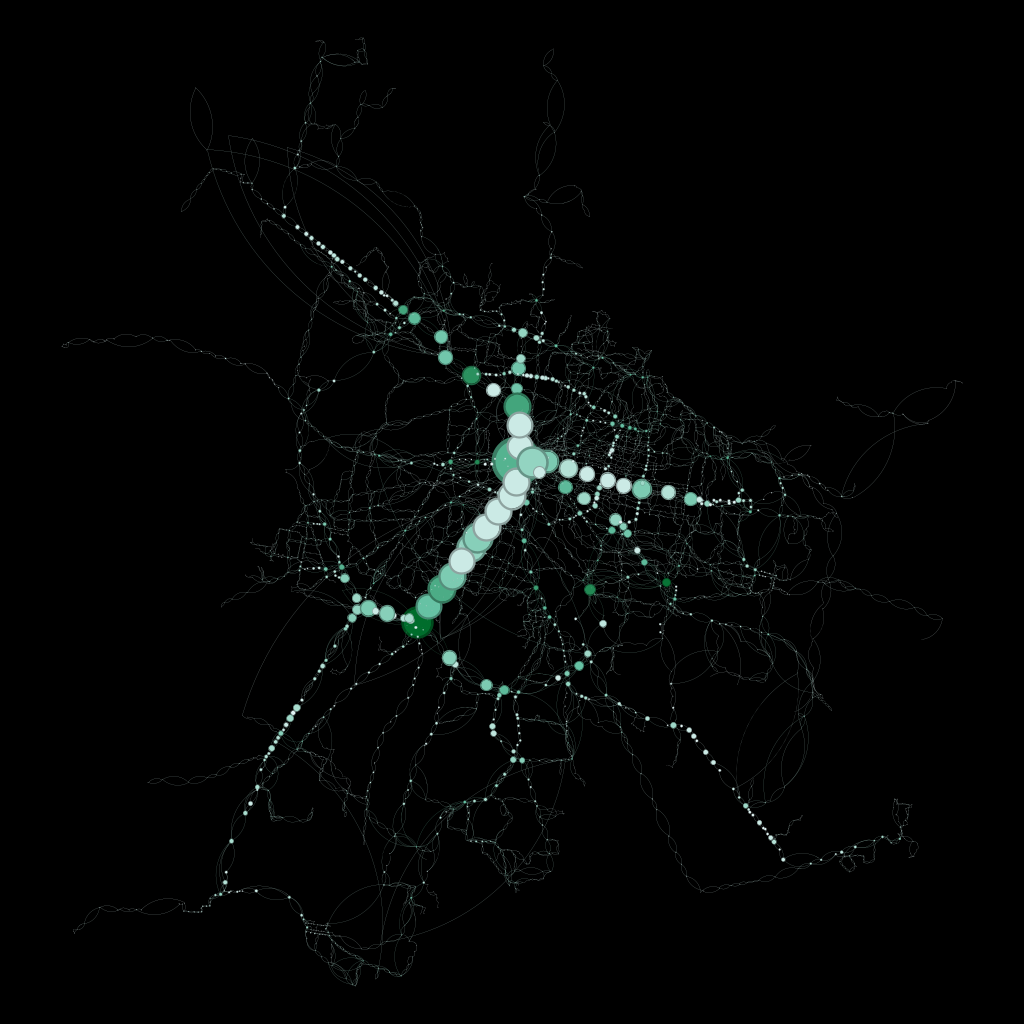
\includegraphics[width=\linewidth,height=0.62\textheight,keepaspectratio]{figuras/l_centralidad.png}
    \end{column}
    \begin{column}{0.38\linewidth}
      \textbf{Lectura}

      Los nodos centrales no son equivalentes: algunos concentran accesibilidad, otros conectan corredores y otros acumulan influencia por vecindad.

      \thinrule

      El Centro Histórico concentra accesibilidad e intermediación; las grandes avenidas reúnen volumen y Mariano Otero aparece como eje de influencia estructural.
    \end{column}
  \end{columns}
\end{frame}

% 20
\begin{frame}{Robustez en \(L\)}
  \begin{columns}[T,onlytextwidth]
    \begin{column}{0.57\linewidth}
      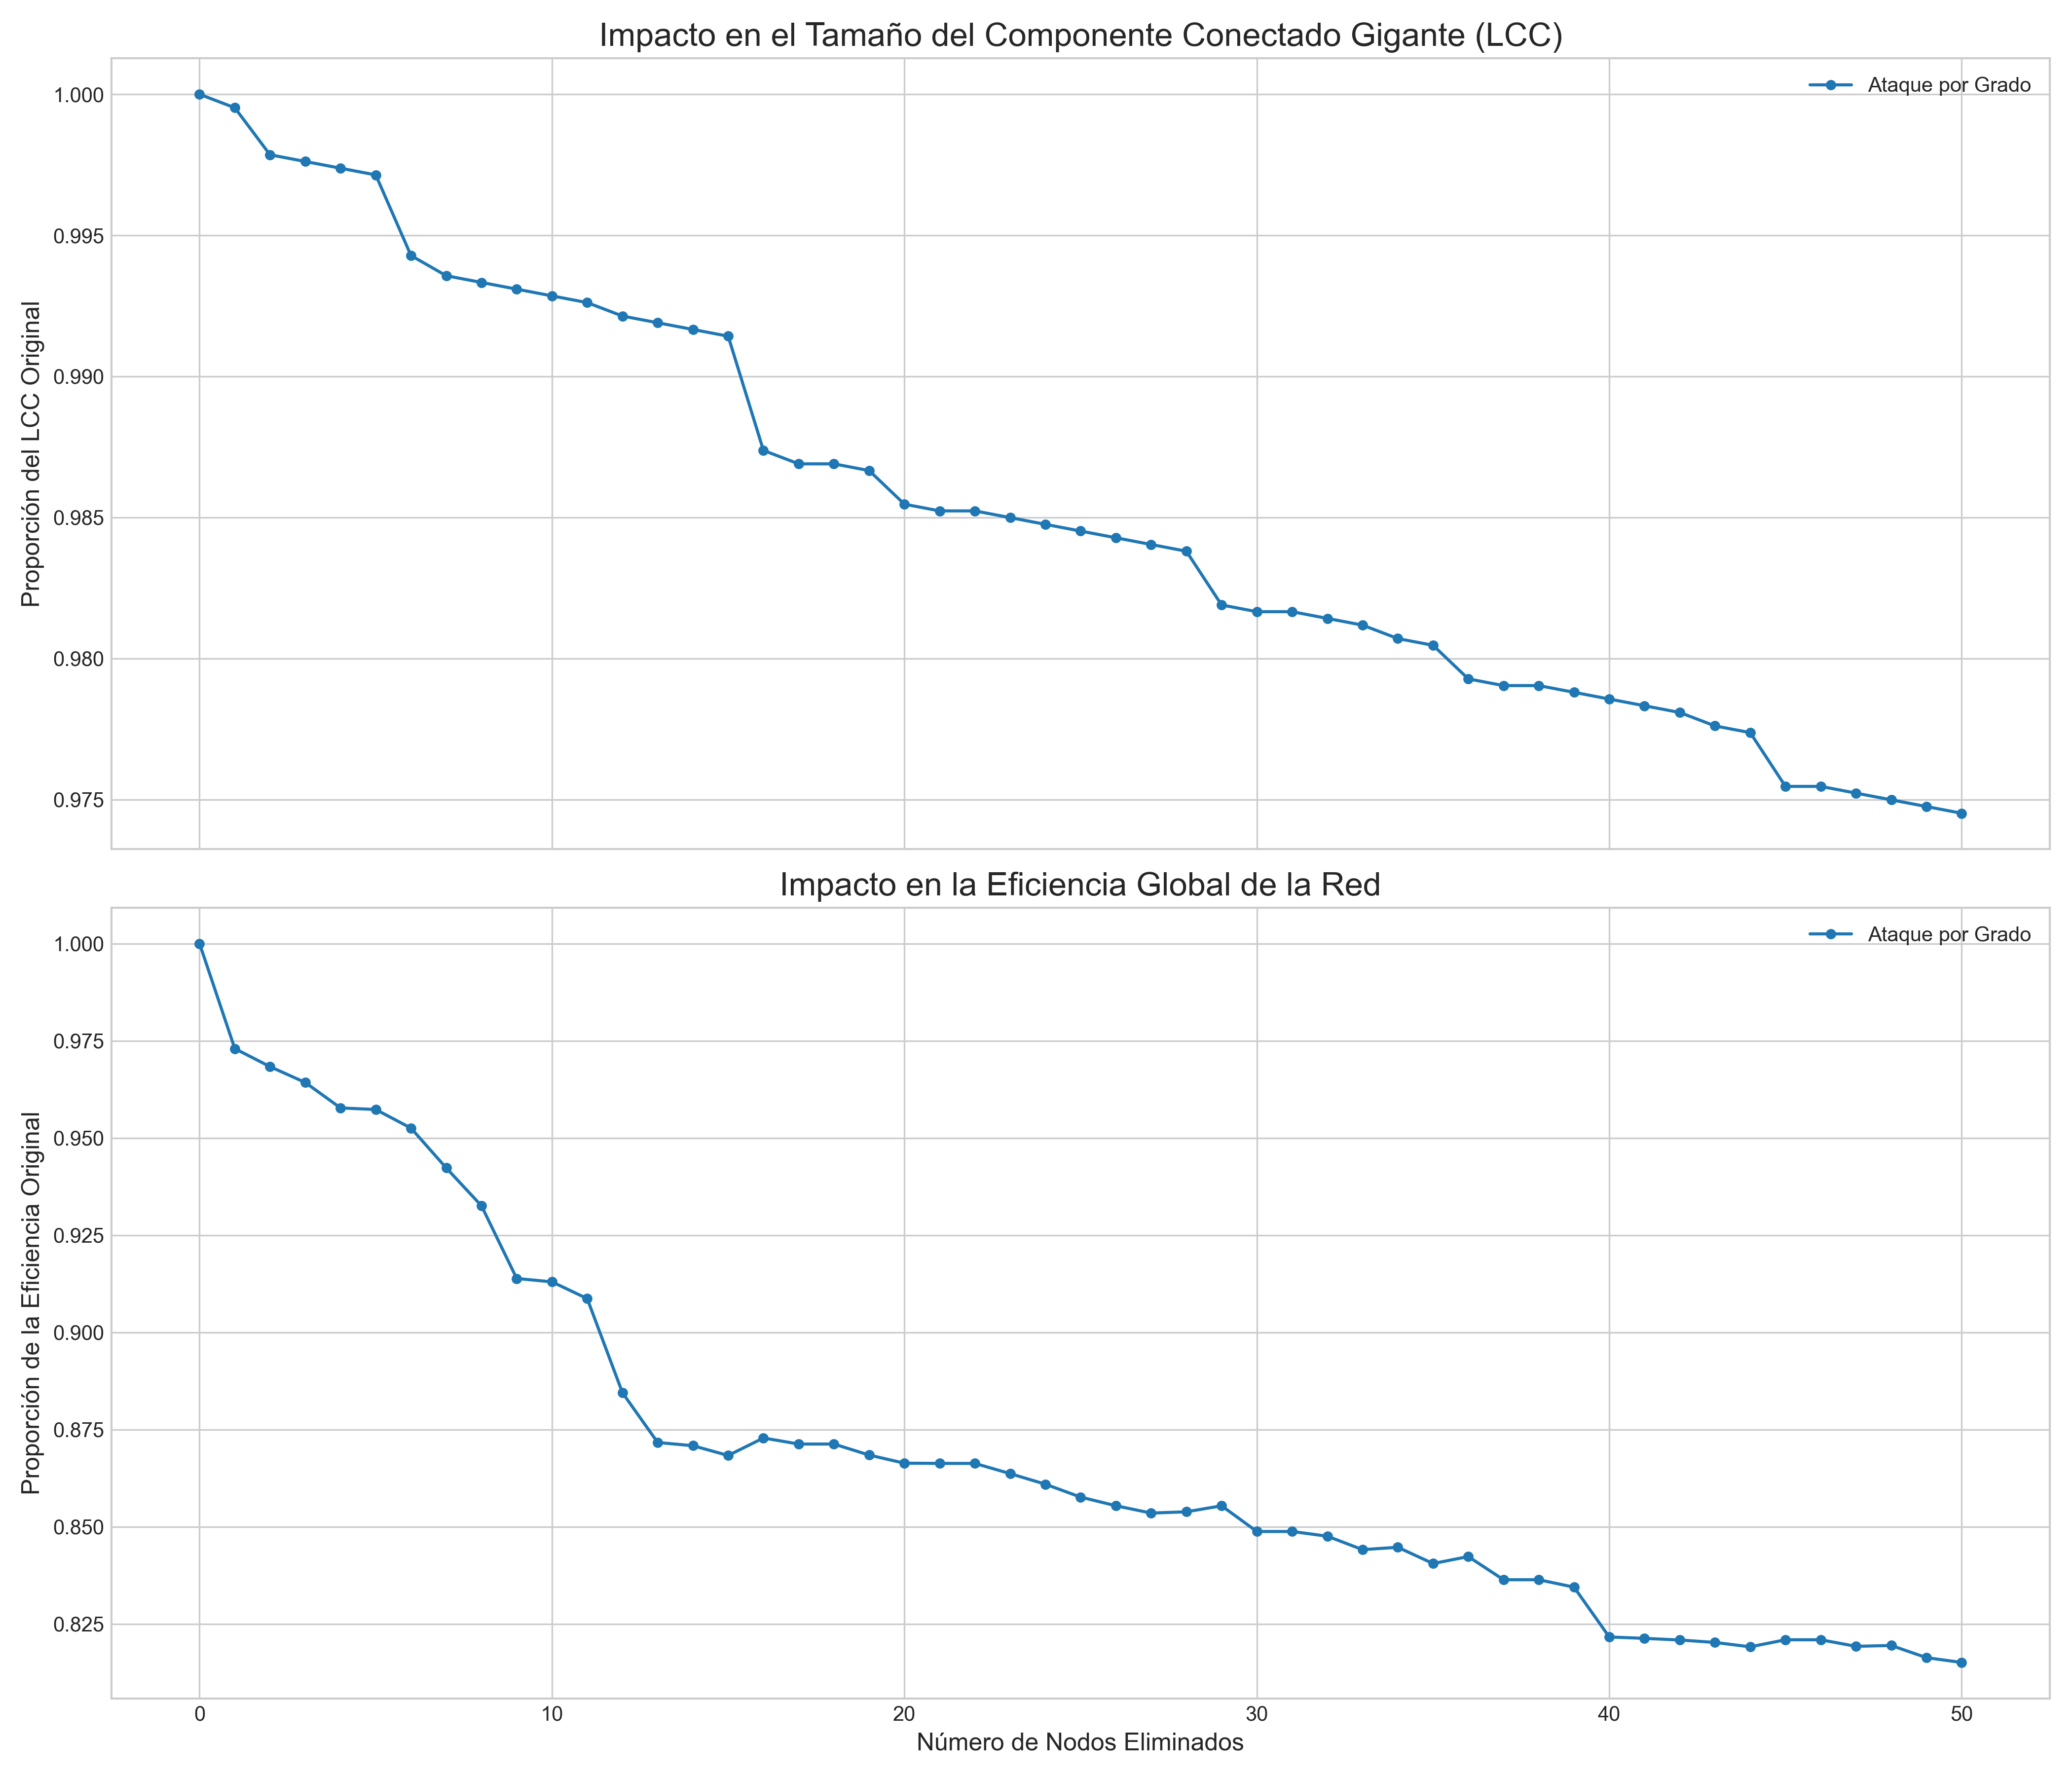
\includegraphics[width=\linewidth,height=0.62\textheight,keepaspectratio]{figuras/l_robustez.png}
    \end{column}
    \begin{column}{0.38\linewidth}
      \small
      \textbf{Ataque dirigido}\par
      LCC \(97.45\%\), eficiencia \(81.50\%\).

      \vspace{0.16cm}
      \textbf{Fallo aleatorio}\par
      LCC medio \(98.23\%\), eficiencia media \(97.17\%\).

      \thinrule
      La eficiencia es más sensible que el tamaño de la componente gigante.
    \end{column}
  \end{columns}
\end{frame}

% 21
\begin{frame}{Resultados en \(P\): servicio}
  \begin{tabularx}{\linewidth}{@{}>{\bfseries}p{0.25\linewidth}X@{}}
    Tamaño & \(4{,}203\) vértices y \(385{,}225\) aristas no dirigidas. \\
    Densidad & \(0.0436\): casi dos órdenes de magnitud mayor que en \(L\). \\
    Agrupamiento & \(0.4085\): alta formación de cliques por rutas compartidas. \\
    Diámetro & \(6\): pocos saltos topológicos entre zonas. \\
    Camino medio & \(2.41\): estructura funcional compacta. \\
    Eficiencia global & \(0.4476\): mayor accesibilidad topológica que en \(L\). \\
  \end{tabularx}

  \thinrule
  Los supernodos 264, 262 y 698 del hipercentro concentran centralidad de servicio; el 264 ocupa el primer lugar en las cuatro métricas y reúne al menos 30 rutas.
\end{frame}

% 22
\begin{frame}{Comunidades en \(P\)}
  \begin{columns}[T,onlytextwidth]
    \begin{column}{0.57\linewidth}
      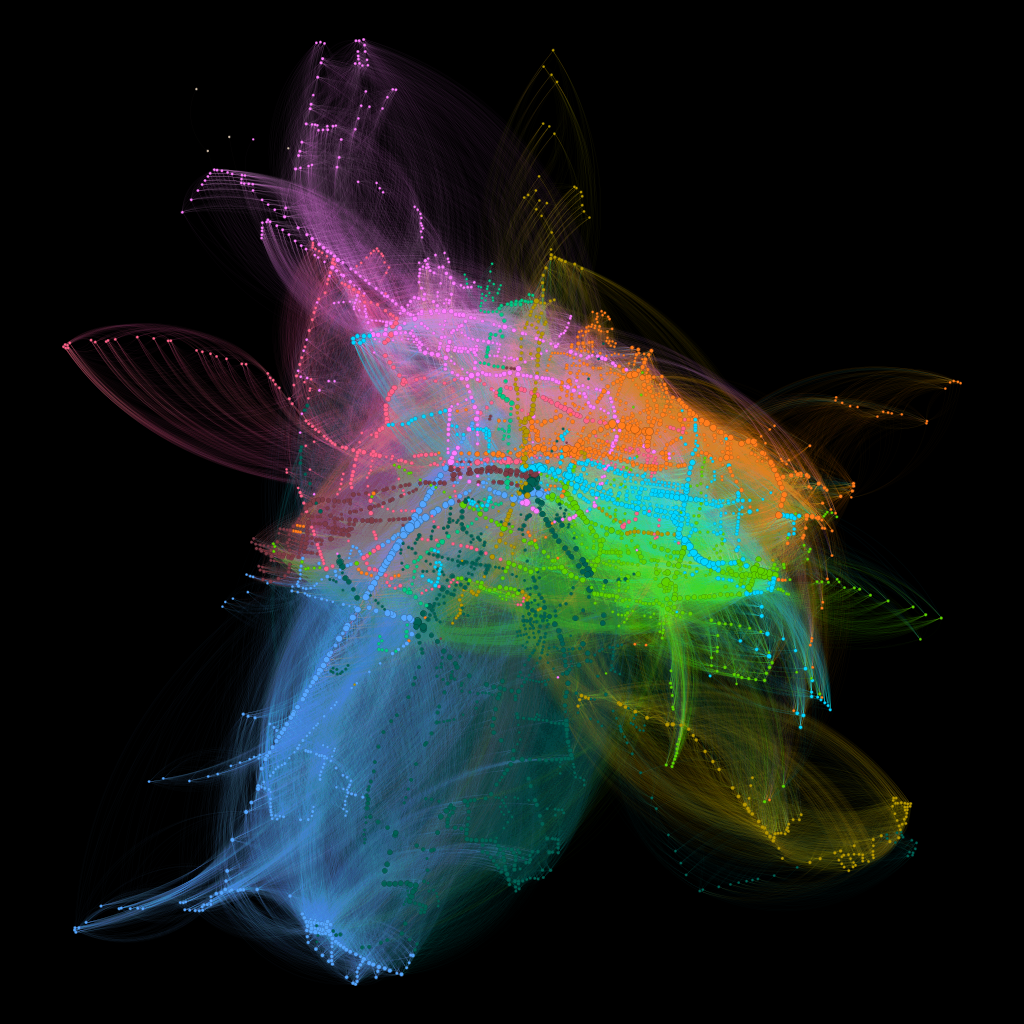
\includegraphics[width=\linewidth,height=0.62\textheight,keepaspectratio]{figuras/p_comunidades.png}
    \end{column}
    \begin{column}{0.38\linewidth}
      \textbf{Resultado}

      Louvain detecta \(11\) comunidades con modularidad \(0.54\).

      \thinrule

      El \(67\%\) de los supernodos queda en las cinco comunidades mayores, lo que sugiere concentración funcional del servicio.
    \end{column}
  \end{columns}
\end{frame}

% 23
\begin{frame}{Robustez en \(P\)}
  \begin{columns}[T,onlytextwidth]
    \begin{column}{0.57\linewidth}
      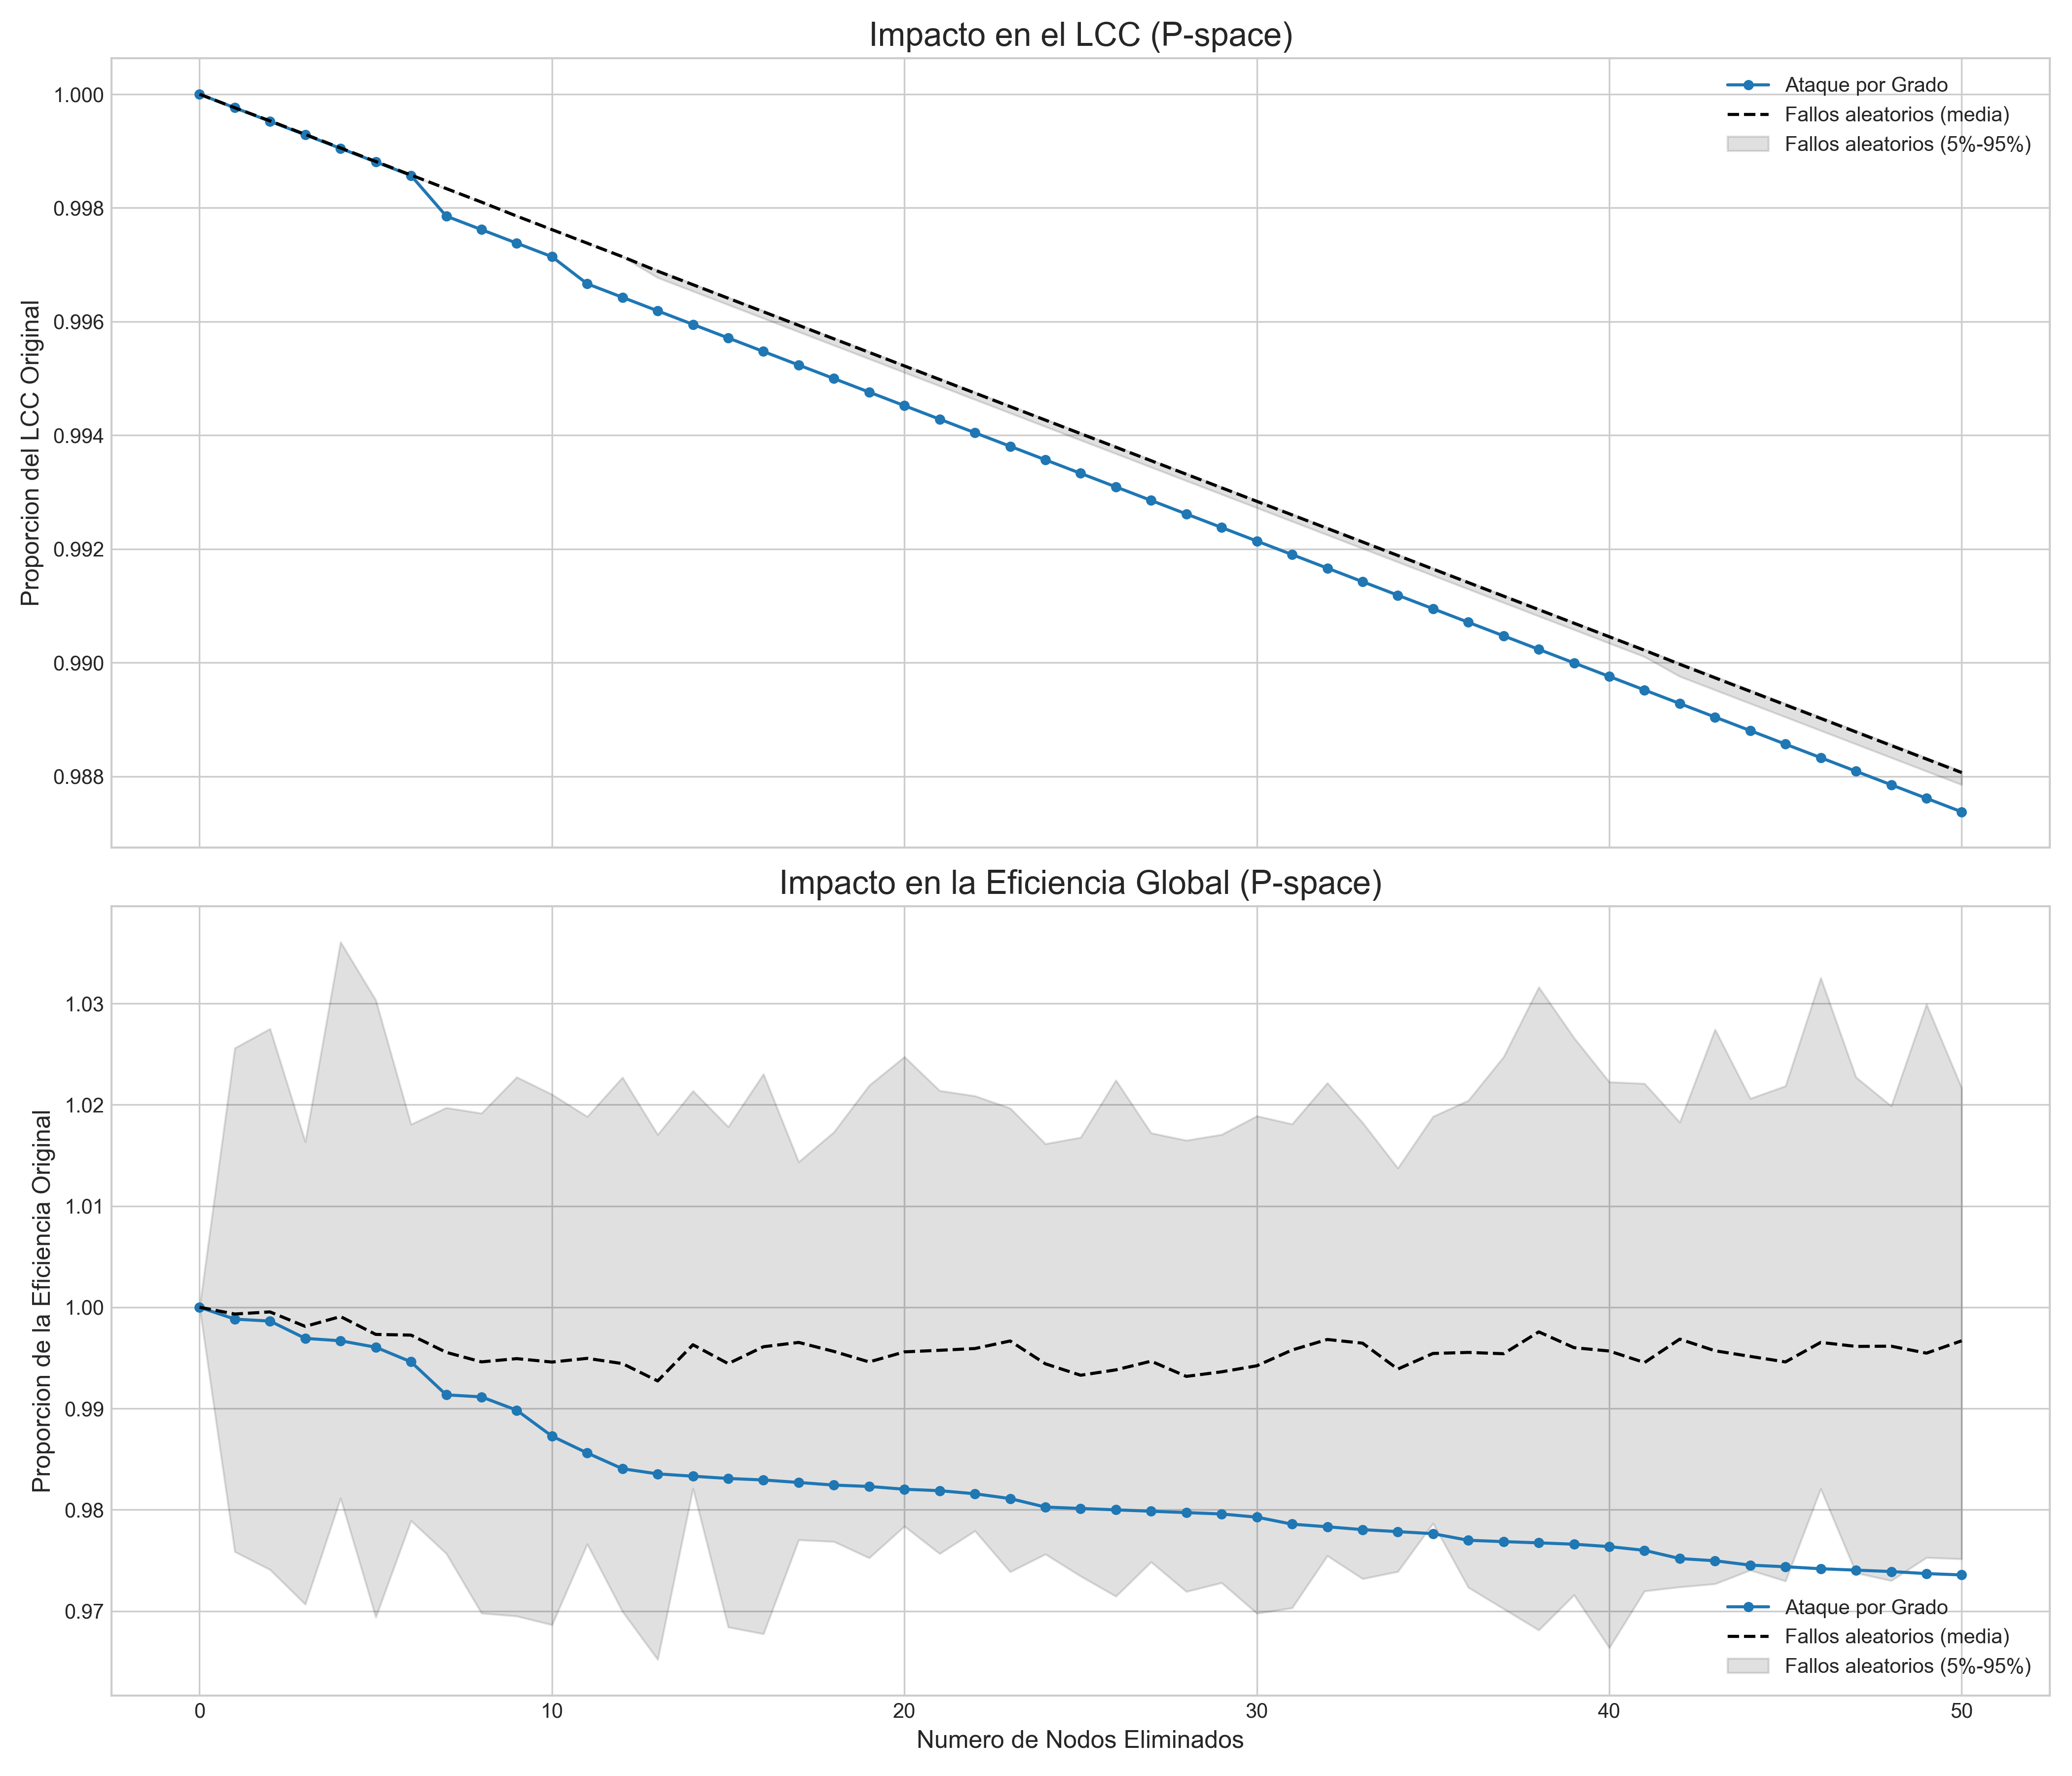
\includegraphics[width=\linewidth,height=0.62\textheight,keepaspectratio]{figuras/p_robustez.png}
    \end{column}
    \begin{column}{0.38\linewidth}
      \small
      \textbf{Ataque dirigido}\par
      LCC \(98.74\%\), eficiencia \(97.36\%\).

      \vspace{0.16cm}
      \textbf{Fallo aleatorio}\par
      LCC medio \(98.80\%\), eficiencia media \(96.93\%\).

      \thinrule
      Bajo el modelo \(P\), la redundancia por rutas compartidas amortigua el ataque dirigido.
    \end{column}
  \end{columns}
\end{frame}

% 24
\begin{frame}{Comparación entre \(L\) y \(P\)}
  \scriptsize
  \begin{tabularx}{\linewidth}{@{}>{\bfseries}p{0.27\linewidth}p{0.20\linewidth}p{0.20\linewidth}X@{}}
    \toprule
    Propiedad & \(L\)-espacio & \(P\)-espacio & Interpretación \\
    \midrule
    Tipo de arista & Consecutividad física & Ruta compartida & Cambia la pregunta modelada. \\
    Densidad & \(0.000486\) & \(0.0436\) & \(P\) es mucho más denso. \\
    Diámetro & \(77\) & \(6\) & El servicio reduce distancias topológicas. \\
    Ataque dirigido, eficiencia & \(81.50\%\) & \(97.36\%\) & La infraestructura pierde más eficiencia. \\
    Fallo aleatorio, eficiencia & \(97.17\%\) & \(96.93\%\) & Los fallos no dirigidos son menos diferenciadores. \\
    \bottomrule
  \end{tabularx}

  \normalsize
  \thinrule
  La evidencia respalda la tesis dentro del modelo construido: la misma red empírica produce diagnósticos distintos según la proyección usada.
\end{frame}

% 25
\begin{frame}{Sensibilidad del modelado}
  \begin{tabularx}{\linewidth}{@{}>{\bfseries}p{0.26\linewidth}X@{}}
    Consolidación espacial & Se evalúan radios de \(75\), \(100\), \(125\) y \(150\) m. \\
    Construcción de \(P\) & Se compara una clique por línea completa (\texttt{route\_id}) frente a una clique por corrida específica (\texttt{trip\_id}). \\
    Hallazgo estable & La red física conserva componente gigante, pero la eficiencia bajo falla es más sensible. \\
    Hallazgo sensible & Las magnitudes de servicio dependen de si el modelo permite permanecer en la misma línea o exige coincidir con una corrida específica. \\
  \end{tabularx}

  \thinrule
  Por ello, las conclusiones cualitativas se reportan junto con rangos y supuestos de construcción.
\end{frame}

% 26
\begin{frame}{Escenarios de intervención modelada}
  \begin{columns}[T,onlytextwidth]
    \begin{column}{0.52\linewidth}
      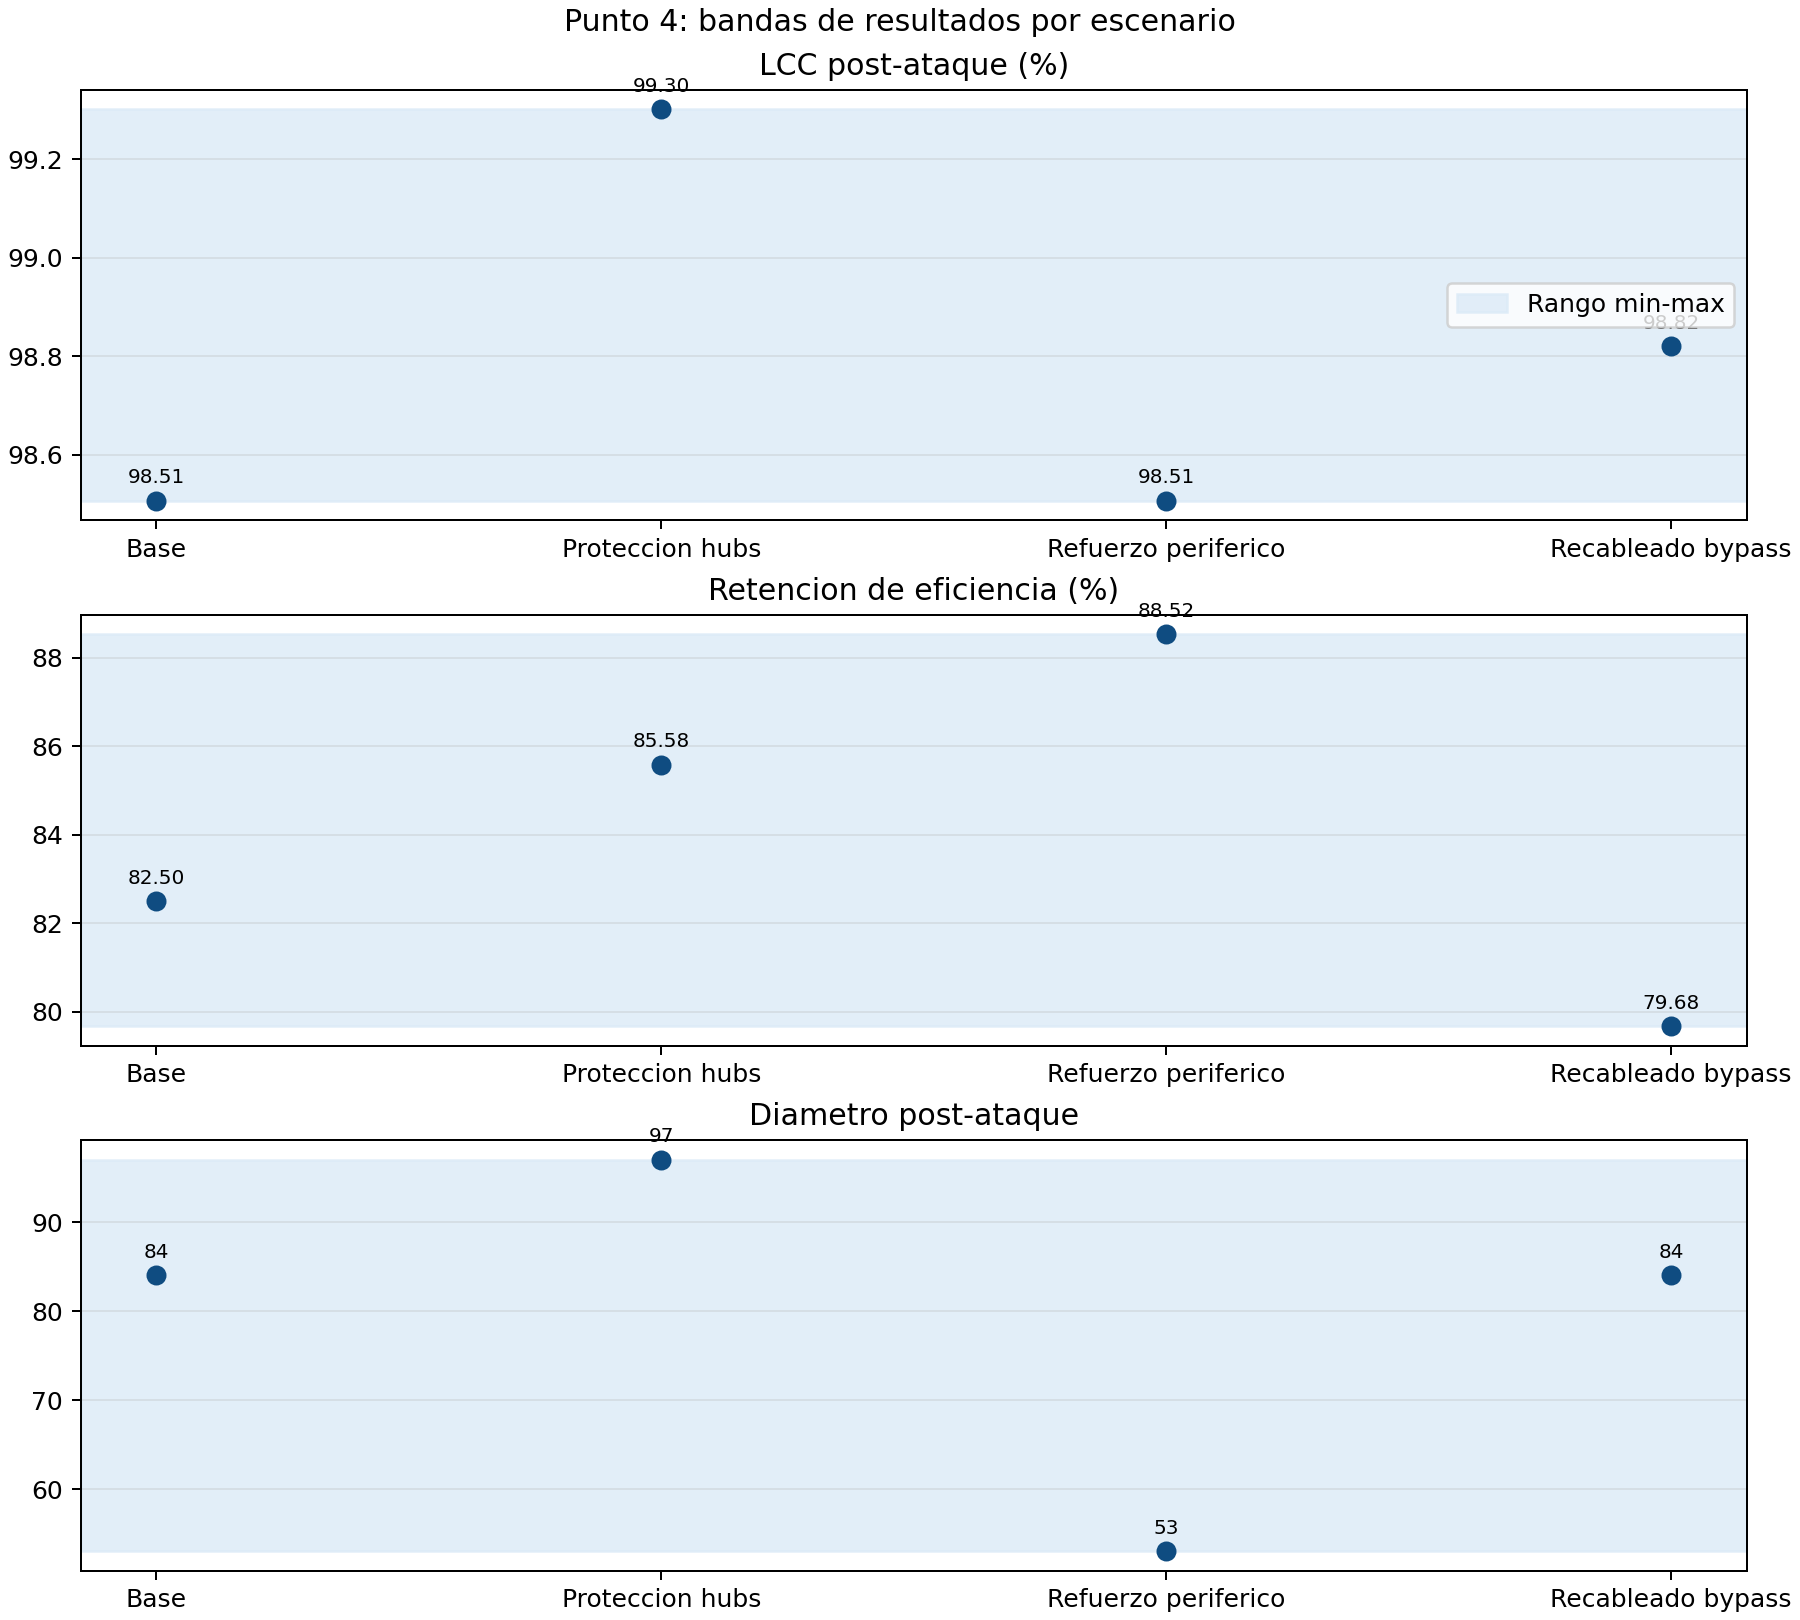
\includegraphics[width=\linewidth,height=0.62\textheight,keepaspectratio]{figuras/intervenciones.png}
    \end{column}
    \begin{column}{0.44\linewidth}
      \scriptsize
      \textbf{Operaciones simuladas}\par
      Proteger nodos concentradores; agregar enlaces periféricos; abrir derivaciones locales alrededor de nodos cargados.

      \vspace{0.12cm}
      \textbf{Protección de nodos concentradores}\par
      LCC \(99.30\%\), eficiencia \(85.58\%\).

      \vspace{0.11cm}
      \textbf{Refuerzo periférico}\par
      LCC \(98.51\%\), eficiencia \(88.52\%\).

      \vspace{0.11cm}
      \textbf{Conexiones de derivación locales}\par
      LCC \(98.82\%\), eficiencia \(79.68\%\).

      \normalsize
      \thinrule
      La intervención más conveniente depende de si se prioriza conectividad global, eficiencia o reducción del peor recorrido interno postataque.
    \end{column}
  \end{columns}
\end{frame}

% 27
\begin{frame}{Reproducibilidad}
  Los insumos y el código quedan separados: el repositorio de la tesis contiene scripts, tablas y figuras; el respaldo GTFS conserva el paquete usado como fuente empírica.

  \vspace{0.3cm}
  \begin{columns}[T,onlytextwidth]
    \begin{column}{0.47\linewidth}
      \centering
      \qrcode[height=2.75cm]{https://github.com/Betancourt1/tesis}

      \vspace{0.18cm}
      \textbf{Repositorio de tesis}

      {\scriptsize\url{https://github.com/Betancourt1/tesis}}
    \end{column}
    \begin{column}{0.47\linewidth}
      \centering
      \qrcode[height=2.75cm]{https://github.com/Betancourt1/gtfs-amg-20240312}

      \vspace{0.18cm}
      \textbf{Respaldo GTFS}

      {\scriptsize\url{https://github.com/Betancourt1/gtfs-amg-20240312}}
    \end{column}
  \end{columns}
\end{frame}

% 28
\begin{frame}{Cierre}
  \claim{La misma red empírica produce diagnósticos distintos según la proyección matemática usada.}

  \vspace{0.3cm}
  \begin{tabularx}{\linewidth}{@{}>{\bfseries}p{0.25\linewidth}X@{}}
    Matemáticamente & \(L\), \(P\), \(C\) y \(B\) son proyecciones de una estructura de transporte común. \\
    Empíricamente & \(L\) es disperso y sensible en eficiencia ante ataque dirigido; \(P\) es denso y retiene conectividad funcional. \\
    Metodológicamente & La conclusión debe leerse bajo sus supuestos: topología, GTFS estático y construcción por zonas consolidadas. \\
  \end{tabularx}

  \thinrule
  La aportación del proyecto es convertir un sistema urbano complejo en objetos comparables, medibles y reproducibles mediante teoría de grafos.
\end{frame}

\end{document}
